
%% bare_conf.tex
%% V1.3
%% 2007/01/11
%% by Michael Shell
%% See:
%% http://www.michaelshell.org/
%% for current contact information.
%%
%% This is a skeleton file demonstrating the use of IEEEtran.cls
%% (requires IEEEtran.cls version 1.7 or later) with an IEEE conference paper.
%%
%% Support sites:
%% http://www.michaelshell.org/tex/ieeetran/
%% http://www.ctan.org/tex-archive/macros/latex/contrib/IEEEtran/
%% and
%% http://www.ieee.org/

%%*************************************************************************
%% Legal Notice:
%% This code is offered as-is without any warranty either expressed or
%% implied; without even the implied warranty of MERCHANTABILITY or
%% FITNESS FOR A PARTICULAR PURPOSE! 
%% User assumes all risk.
%% In no event shall IEEE or any contributor to this code be liable for
%% any damages or losses, including, but not limited to, incidental,
%% consequential, or any other damages, resulting from the use or misuse
%% of any information contained here.
%%
%% All comments are the opinions of their respective authors and are not
%% necessarily endorsed by the IEEE.
%%
%% This work is distributed under the LaTeX Project Public License (LPPL)
%% ( http://www.latex-project.org/ ) version 1.3, and may be freely used,
%% distributed and modified. A copy of the LPPL, version 1.3, is included
%% in the base LaTeX documentation of all distributions of LaTeX released
%% 2003/12/01 or later.
%% Retain all contribution notices and credits.
%% ** Modified files should be clearly indicated as such, including  **
%% ** renaming them and changing author support contact information. **
%%
%% File list of work: IEEEtran.cls, IEEEtran_HOWTO.pdf, bare_adv.tex,
%%                    bare_conf.tex, bare_jrnl.tex, bare_jrnl_compsoc.tex
%%*************************************************************************

% *** Authors should verify (and, if needed, correct) their LaTeX system  ***
% *** with the testflow diagnostic prior to trusting their LaTeX platform ***
% *** with production work. IEEE's font choices can trigger bugs that do  ***
% *** not appear when using other class files.                            ***
% The testflow support page is at:
% http://www.michaelshell.org/tex/testflow/



% Note that the a4paper option is mainly intended so that authors in
% countries using A4 can easily print to A4 and see how their papers will
% look in print - the typesetting of the document will not typically be
% affected with changes in paper size (but the bottom and side margins will).
% Use the testflow package mentioned above to verify correct handling of
% both paper sizes by the user's LaTeX system.
%
% Also note that the "draftcls" or "draftclsnofoot", not "draft", option
% should be used if it is desired that the figures are to be displayed in
% draft mode.
%
\documentclass[10pt, conference, compsocconf]{IEEEtran}
% Add the compsocconf option for Computer Society conferences.
%
% If IEEEtran.cls has not been installed into the LaTeX system files,
% manually specify the path to it like:
% \documentclass[conference]{../sty/IEEEtran}

\usepackage{rotating}

% Some very useful LaTeX packages include:
% (uncomment the ones you want to load)


% *** MISC UTILITY PACKAGES ***
%
%\usepackage{ifpdf}
% Heiko Oberdiek's ifpdf.sty is very useful if you need conditional
% compilation based on whether the output is pdf or dvi.
% usage:
% \ifpdf
%   % pdf code
% \else
%   % dvi code
% \fi
% The latest version of ifpdf.sty can be obtained from:
% http://www.ctan.org/tex-archive/macros/latex/contrib/oberdiek/
% Also, note that IEEEtran.cls V1.7 and later provides a builtin
% \ifCLASSINFOpdf conditional that works the same way.
% When switching from latex to pdflatex and vice-versa, the compiler may
% have to be run twice to clear warning/error messages.






% *** CITATION PACKAGES ***
%
%\usepackage{cite}
% cite.sty was written by Donald Arseneau
% V1.6 and later of IEEEtran pre-defines the format of the cite.sty package
% \cite{} output to follow that of IEEE. Loading the cite package will
% result in citation numbers being automatically sorted and properly
% "compressed/ranged". e.g., [1], [9], [2], [7], [5], [6] without using
% cite.sty will become [1], [2], [5]--[7], [9] using cite.sty. cite.sty's
% \cite will automatically add leading space, if needed. Use cite.sty's
% noadjust option (cite.sty V3.8 and later) if you want to turn this off.
% cite.sty is already installed on most LaTeX systems. Be sure and use
% version 4.0 (2003-05-27) and later if using hyperref.sty. cite.sty does
% not currently provide for hyperlinked citations.
% The latest version can be obtained at:
% http://www.ctan.org/tex-archive/macros/latex/contrib/cite/
% The documentation is contained in the cite.sty file itself.






% *** GRAPHICS RELATED PACKAGES ***
%
\ifCLASSINFOpdf
  % \usepackage[pdftex]{graphicx}
  % declare the path(s) where your graphic files are
  % \graphicspath{{../pdf/}{../jpeg/}}
  % and their extensions so you won't have to specify these with
  % every instance of \includegraphics
  % \DeclareGraphicsExtensions{.pdf,.jpeg,.png}
\else
  % or other class option (dvipsone, dvipdf, if not using dvips). graphicx
  % will default to the driver specified in the system graphics.cfg if no
  % driver is specified.
  % \usepackage[dvips]{graphicx}
  % declare the path(s) where your graphic files are
  % \graphicspath{{../eps/}}
  % and their extensions so you won't have to specify these with
  % every instance of \includegraphics
  % \DeclareGraphicsExtensions{.eps}
\fi
% graphicx was written by David Carlisle and Sebastian Rahtz. It is
% required if you want graphics, photos, etc. graphicx.sty is already
% installed on most LaTeX systems. The latest version and documentation can
% be obtained at: 
% http://www.ctan.org/tex-archive/macros/latex/required/graphics/
% Another good source of documentation is "Using Imported Graphics in
% LaTeX2e" by Keith Reckdahl which can be found as epslatex.ps or
% epslatex.pdf at: http://www.ctan.org/tex-archive/info/
%
% latex, and pdflatex in dvi mode, support graphics in encapsulated
% postscript (.eps) format. pdflatex in pdf mode supports graphics
% in .pdf, .jpeg, .png and .mps (metapost) formats. Users should ensure
% that all non-photo figures use a vector format (.eps, .pdf, .mps) and
% not a bitmapped formats (.jpeg, .png). IEEE frowns on bitmapped formats
% which can result in "jaggedy"/blurry rendering of lines and letters as
% well as large increases in file sizes.
%
% You can find documentation about the pdfTeX application at:
% http://www.tug.org/applications/pdftex





% *** MATH PACKAGES ***
%
%\usepackage[cmex10]{amsmath}
% A popular package from the American Mathematical Society that provides
% many useful and powerful commands for dealing with mathematics. If using
% it, be sure to load this package with the cmex10 option to ensure that
% only type 1 fonts will utilized at all point sizes. Without this option,
% it is possible that some math symbols, particularly those within
% footnotes, will be rendered in bitmap form which will result in a
% document that can not be IEEE Xplore compliant!
%
% Also, note that the amsmath package sets \interdisplaylinepenalty to 10000
% thus preventing page breaks from occurring within multiline equations. Use:
%\interdisplaylinepenalty=2500
% after loading amsmath to restore such page breaks as IEEEtran.cls normally
% does. amsmath.sty is already installed on most LaTeX systems. The latest
% version and documentation can be obtained at:
% http://www.ctan.org/tex-archive/macros/latex/required/amslatex/math/





% *** SPECIALIZED LIST PACKAGES ***
%
%\usepackage{algorithmic}
% algorithmic.sty was written by Peter Williams and Rogerio Brito.
% This package provides an algorithmic environment fo describing algorithms.
% You can use the algorithmic environment in-text or within a figure
% environment to provide for a floating algorithm. Do NOT use the algorithm
% floating environment provided by algorithm.sty (by the same authors) or
% algorithm2e.sty (by Christophe Fiorio) as IEEE does not use dedicated
% algorithm float types and packages that provide these will not provide
% correct IEEE style captions. The latest version and documentation of
% algorithmic.sty can be obtained at:
% http://www.ctan.org/tex-archive/macros/latex/contrib/algorithms/
% There is also a support site at:
% http://algorithms.berlios.de/index.html
% Also of interest may be the (relatively newer and more customizable)
% algorithmicx.sty package by Szasz Janos:
% http://www.ctan.org/tex-archive/macros/latex/contrib/algorithmicx/




% *** ALIGNMENT PACKAGES ***
%
%\usepackage{array}
% Frank Mittelbach's and David Carlisle's array.sty patches and improves
% the standard LaTeX2e array and tabular environments to provide better
% appearance and additional user controls. As the default LaTeX2e table
% generation code is lacking to the point of almost being broken with
% respect to the quality of the end results, all users are strongly
% advised to use an enhanced (at the very least that provided by array.sty)
% set of table tools. array.sty is already installed on most systems. The
% latest version and documentation can be obtained at:
% http://www.ctan.org/tex-archive/macros/latex/required/tools/


%\usepackage{mdwmath}
%\usepackage{mdwtab}
% Also highly recommended is Mark Wooding's extremely powerful MDW tools,
% especially mdwmath.sty and mdwtab.sty which are used to format equations
% and tables, respectively. The MDWtools set is already installed on most
% LaTeX systems. The lastest version and documentation is available at:
% http://www.ctan.org/tex-archive/macros/latex/contrib/mdwtools/


% IEEEtran contains the IEEEeqnarray family of commands that can be used to
% generate multiline equations as well as matrices, tables, etc., of high
% quality.


%\usepackage{eqparbox}
% Also of notable interest is Scott Pakin's eqparbox package for creating
% (automatically sized) equal width boxes - aka "natural width parboxes".
% Available at:
% http://www.ctan.org/tex-archive/macros/latex/contrib/eqparbox/





% *** SUBFIGURE PACKAGES ***
%\usepackage[tight,footnotesize]{subfigure}
% subfigure.sty was written by Steven Douglas Cochran. This package makes it
% easy to put subfigures in your figures. e.g., "Figure 1a and 1b". For IEEE
% work, it is a good idea to load it with the tight package option to reduce
% the amount of white space around the subfigures. subfigure.sty is already
% installed on most LaTeX systems. The latest version and documentation can
% be obtained at:
% http://www.ctan.org/tex-archive/obsolete/macros/latex/contrib/subfigure/
% subfigure.sty has been superceeded by subfig.sty.



%\usepackage[caption=false]{caption}
%\usepackage[font=footnotesize]{subfig}
% subfig.sty, also written by Steven Douglas Cochran, is the modern
% replacement for subfigure.sty. However, subfig.sty requires and
% automatically loads Axel Sommerfeldt's caption.sty which will override
% IEEEtran.cls handling of captions and this will result in nonIEEE style
% figure/table captions. To prevent this problem, be sure and preload
% caption.sty with its "caption=false" package option. This is will preserve
% IEEEtran.cls handing of captions. Version 1.3 (2005/06/28) and later 
% (recommended due to many improvements over 1.2) of subfig.sty supports
% the caption=false option directly:
%\usepackage[caption=false,font=footnotesize]{subfig}
%
% The latest version and documentation can be obtained at:
% http://www.ctan.org/tex-archive/macros/latex/contrib/subfig/
% The latest version and documentation of caption.sty can be obtained at:
% http://www.ctan.org/tex-archive/macros/latex/contrib/caption/




% *** FLOAT PACKAGES ***
%
%\usepackage{fixltx2e}
% fixltx2e, the successor to the earlier fix2col.sty, was written by
% Frank Mittelbach and David Carlisle. This package corrects a few problems
% in the LaTeX2e kernel, the most notable of which is that in current
% LaTeX2e releases, the ordering of single and double column floats is not
% guaranteed to be preserved. Thus, an unpatched LaTeX2e can allow a
% single column figure to be placed prior to an earlier double column
% figure. The latest version and documentation can be found at:
% http://www.ctan.org/tex-archive/macros/latex/base/



%\usepackage{stfloats}
% stfloats.sty was written by Sigitas Tolusis. This package gives LaTeX2e
% the ability to do double column floats at the bottom of the page as well
% as the top. (e.g., "\begin{figure*}[!b]" is not normally possible in
% LaTeX2e). It also provides a command:
%\fnbelowfloat
% to enable the placement of footnotes below bottom floats (the standard
% LaTeX2e kernel puts them above bottom floats). This is an invasive package
% which rewrites many portions of the LaTeX2e float routines. It may not work
% with other packages that modify the LaTeX2e float routines. The latest
% version and documentation can be obtained at:
% http://www.ctan.org/tex-archive/macros/latex/contrib/sttools/
% Documentation is contained in the stfloats.sty comments as well as in the
% presfull.pdf file. Do not use the stfloats baselinefloat ability as IEEE
% does not allow \baselineskip to stretch. Authors submitting work to the
% IEEE should note that IEEE rarely uses double column equations and
% that authors should try to avoid such use. Do not be tempted to use the
% cuted.sty or midfloat.sty packages (also by Sigitas Tolusis) as IEEE does
% not format its papers in such ways.





% *** PDF, URL AND HYPERLINK PACKAGES ***
%
%\usepackage{url}
% url.sty was written by Donald Arseneau. It provides better support for
% handling and breaking URLs. url.sty is already installed on most LaTeX
% systems. The latest version can be obtained at:
% http://www.ctan.org/tex-archive/macros/latex/contrib/misc/
% Read the url.sty source comments for usage information. Basically,
% \url{my_url_here}.





% *** Do not adjust lengths that control margins, column widths, etc. ***
% *** Do not use packages that alter fonts (such as pslatex).         ***
% There should be no need to do such things with IEEEtran.cls V1.6 and later.
% (Unless specifically asked to do so by the journal or conference you plan
% to submit to, of course. )


% correct bad hyphenation here
\hyphenation{op-tical net-works semi-conduc-tor}

\usepackage{alltt}
\usepackage{hyperref}
\hypersetup{pdfborder={0 0 0}}

\usepackage{balance}

\clubpenalty = 10000
\widowpenalty = 10000
\displaywidowpenalty = 10000

\begin{document}
%
% paper title
% can use linebreaks \\ within to get better formatting as desired
\title{Active Code Completion}


% author names and affiliations
% use a multiple column layout for up to two different
% affiliations

\author{\IEEEauthorblockN{Cyrus Omar, YoungSeok Yoon, Thomas D. LaToza, Brad A. Myers}
\IEEEauthorblockA{Carnegie Mellon University, 
Pittsburgh, PA, USA\\
\small{{\{comar,youngseok,tlatoza,bam\}$@$cs.cmu.edu}}\\
\small{\texttt{\url{http://www.cs.cmu.edu/~NatProg/graphite.html}}}}
}

% conference papers do not typically use \thanks and this command
% is locked out in conference mode. If really needed, such as for
% the acknowledgment of grants, issue a \IEEEoverridecommandlockouts
% after \documentclass

% for over three affiliations, or if they all won't fit within the width
% of the page, use this alternative format:
% 
%\author{\IEEEauthorblockN{Michael Shell\IEEEauthorrefmark{1},
%Homer Simpson\IEEEauthorrefmark{2},
%James Kirk\IEEEauthorrefmark{3}, 
%Montgomery Scott\IEEEauthorrefmark{3} and
%Eldon Tyrell\IEEEauthorrefmark{4}}
%\IEEEauthorblockA{\IEEEauthorrefmark{1}School of Electrical and Computer Engineering\\
%Georgia Institute of Technology,
%Atlanta, Georgia 30332--0250\\ Email: see http://www.michaelshell.org/contact.html}
%\IEEEauthorblockA{\IEEEauthorrefmark{2}Twentieth Century Fox, Springfield, USA\\
%Email: homer@thesimpsons.com}
%\IEEEauthorblockA{\IEEEauthorrefmark{3}Starfleet Academy, San Francisco, California 96678-2391\\
%Telephone: (800) 555--1212, Fax: (888) 555--1212}
%\IEEEauthorblockA{\IEEEauthorrefmark{4}Tyrell Inc., 123 Replicant Street, Los Angeles, California 90210--4321}}




% use for special paper notices
%\IEEEspecialpapernotice{(Invited Paper)}




% make the title area
\maketitle


\begin{abstract}
Code completion menus have replaced standalone API browsers for most developers because they are more tightly  integrated into the development workflow. Refinements to the code completion menu that incorporate additional sources of information have similarly been shown to be valuable, even relative to standalone counterparts offering similar functionality. In this paper, we describe {\em active code completion}, an architecture that allows library developers to introduce interactive and highly-specialized code generation interfaces, called {\em palettes}, directly into the editor. Using several empirical methods, we examine the contexts in which such a system could be useful, describe the design constraints governing the system architecture as well as particular code completion interfaces, and design one such system, named Graphite, for the Eclipse Java development environment. Using Graphite, we implement a palette for writing regular expressions as our primary  example and conduct a small pilot study. In addition to showing the feasibility of this approach, it provides further evidence in support of the claim that integrating specialized code completion interfaces directly into the editor is valuable to professional developers.
\end{abstract}

\begin{IEEEkeywords}
code completion, development environments

\end{IEEEkeywords}


% For peer review papers, you can put extra information on the cover
% page as needed:
% \ifCLASSOPTIONpeerreview
% \begin{center} \bfseries EDICS Category: 3-BBND \end{center}
% \fi
%
% For peerreview papers, this IEEEtran command inserts a page break and
% creates the second title. It will be ignored for other modes.
\IEEEpeerreviewmaketitle
\section{Introduction}
Software developers today make heavy use of the code completion support found in modern source code editors  \cite{murphy_how_2006}. Most editors provide code completion in the form of a floating menu containing  contextually-relevant variables, fields, methods, types and other code snippets. By navigating and selecting from this menu, developers are able to avoid many common spelling and logic errors, eliminate unnecessary keystrokes and explore unfamiliar APIs without incurring the mental overhead associated with switching to an external documentation tool or API browser.
% The way code completion menus brought documentation systems into the editor, active code completion interfaces bring external tools into the editor.

Several refinements and additions to the code completion menu have previously been suggested in the literature. These have focused on leveraging additional sources of information, such as databases of usage history \cite{robbes_how_2008}\cite{HouPletcher2011}, inheritance information \cite{HouPletcher2011}, API-specific information \cite{HouPletcher2011}\cite{Lee+2008}, partial abbreviations \cite{Han+2009}, examples extracted from code repositories \cite{bruch_learning_2009}\cite{Brandt+2010} and crowdsourced information \cite{mooty_calcite:_2010}\cite{SnipMatch}, to increase the relevance and sophistication of the featured menu items. As with the standard form of code completion, many of these sources of data can also be utilized via external tools (e.g. Calcite \cite{mooty_calcite:_2010} uses information that could already be accessed using the Jadeite \cite{conf/vl/StylosFYM09} tool). Empirical evidence presented in these studies, however, suggests that directly integrating these kinds of tools into the editor is particularly effective. For example, users of the Calcite tool completed 40\% more tasks in a lab study (unfortunately, a Jadeite control group was not included.)

In all of these systems, the code completion interface has remained primarily menu-based. When an item is selected, code is inserted immediately, without further input from the developer. These systems are also difficult to extend: a fixed strategy determines the completions that are available, so library providers cannot directly specify new domain-specific or contextually-relevant logic. 
In this paper we propose a technique called {\it active code completion} that eliminates these restrictions\footnote{Portions of this work previously appeared in a poster abstract \cite{ACC_VLHCC}.}. This  makes developing and integrating a broad array of highly-specialized developer tools directly into the editor, via the familiar code completion command, significantly simpler. This technique is motivated by the evidence discussed above and further evidence provided in this paper that developers prefer, and make more effective use of, tools that do not require leaving the immediate editing environment.

In this paper, we discuss active code completion in the context of object construction. For example, consider the following Java code fragment:

\begin{alltt}
  public Color getDefaultColor() \{
      return \textvisiblespace
\end{alltt}

\begin{figure*}\label{color}
\begin{center}
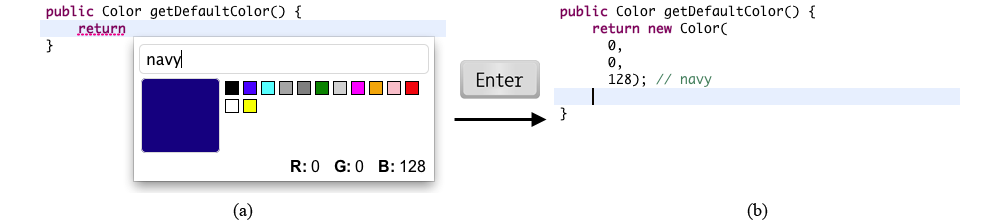
\includegraphics[width=\textwidth]{color_palette.png}\end{center}
\caption{(a) An example code completion palette associated with the \texttt{Color} class. (b) The source code generated by this palette.}
\end{figure*}

If the developer invokes the code completion command at the indicated cursor position (\textvisiblespace), the editor  looks  for a {\it palette definition} associated with the {\it type} of the expression being entered, which in this case is  \verb|Color|. If an associated palette is found, a menu item briefly describing this palette is added to the standard code completion menu. When selected, the corresponding palette is shown, replacing the standard code completion menu. Figure 1a gives an example of a simple palette that may be associated with the \verb|Color| class\footnote{A video demonstrating this process is available from the webpage above.}. 

The developer can interact with such palettes to provide parameters and other information related to her intent, and receive immediate feedback about the effect these choices will have on the behavior of the object being constructed. When this interaction is complete, the palette generates appropriate source code for insertion at the cursor. Figure 1b shows the inserted code after the user presses \textsc{enter}.

In accordance with best practices, we sought to address the following questions before designing and implementing our active code completion system:

\begin{itemize}
\item What {\it specific} use cases exist for this form of active code completion in a professional development setting? 
\item What {\it general} criteria are common to types that would and would not benefit from an associated palette?
\item What are some relevant usability and design criteria for palettes designed to address such use cases?
\item What capabilities must the underlying active code completion system provide to enable these use cases and user interface designs?
\end{itemize}

To help us answer these questions, we conducted a survey of 473 professional developers (Section II). Their responses, along with information gathered from informal interviews and code corpus analyses, revealed a number of non-trivial functional requirements for palette interfaces as well as the underlying active code completion architecture (Section III). Participants also suggested a large number of use cases, demonstrating the broad applicability of this technique. We organize these into several broad categories (Section IV). 

Next, we describe Graphite, an Eclipse plug-in that implements the active code completion architecture for the Java programming language (Section V), allowing Java library developers to associate custom palettes with their own classes. We describe several design choices that we made to satisfy the requirements discovered in our preliminary investigations and briefly examine necessary trade-offs.

Finally, we conducted a pilot lab study with a more complex palette, implemented using Graphite, that assists developers as they write regular expressions (Section VI). The study provides specific evidence in support of the broader claim that highly-specialized tools that are integrated directly with the editing environment are particularly useful. We conclude that active code completion systems like Graphite are useful because they make developing, deploying and discovering such tools fundamentally simpler.

\section{Survey}
To validate our general conceptualization of active code completion, develop concrete criteria to constrain our system and palette designs, and create a list of use cases to justify this effort, we began by conducting a large survey of professional software developers.

% In order to convey the active code completion concept clearly, we came up with three different use cases where we belive the active code completion technique will benefit developers frequently. For each use case, we designed three mockup screenshots and showed them in sequence: before invoking the palette, during the interaction with the palette, and after the palette is closed and code is generated. By doing this, the respondents could understand the concept precisely and give useful feedback relevant to the above questions.
\subsection{Participants}
We recruited participants for this survey\footnote{https://www.surveymonkey.com/s/2GLZP8V} primarily from a popular programming-related discussion forum hosted on the popular website reddit.com \cite{reddit_programming}. An additional 22 participants were computer science graduate students at CMU. 

Recruitment materials in both cases stated that we were seeking developers ``familiar with an object-oriented programming language like Java, C\# or Visual Basic and an integrated development environment like Eclipse or Visual Studio''.
Participants were told that the survey would take approximately 20 minutes to complete, and no reward was offered. Of the 696 people who started the survey, 473 participants (68\%) completed it. We examine the responses from completed surveys only in the analyses below.

\subsection{Familiarity with Programming Languages and Editors}

We first asked participants about their level of familiarity with several programming languages, on a five-point Likert scale\footnote{``None'', ``Somewhat familiar'', ``Familiar'', ``Very familiar'', ``Expert''}. 61.1\% of the participants indicated that they were an expert in at least one language, and an additional 35.7\% were ``very familiar'' with at least one language. On average, participants rated themselves as very familiar with Java, C, C++ and JavaScript, familiar with C\#, Python and PHP and somewhat familiar with Visual Basic and Perl.

We also asked participants to select which integrated development environments (IDEs) and code editors that they were familiar with. The Eclipse IDE was familiar to 87.1\% of participants. This was followed by Visual Studio at 66.0\%, Vi/Vim at 53.7\%, Netbeans at 37.7\%, Emacs at 24.8\% and IntelliJ IDEA at 16.4\%. Participants could also enter ``other'' choices and a number of editors and IDEs were entered, including Xcode, Textmate and Notepad++.

\subsection{Palette Mockups}

%\begin{figure}
%  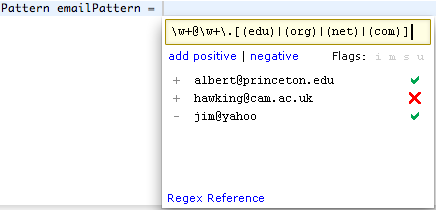
\includegraphics[width=\linewidth]{mockup-palette-small.png}
%  \caption{An example mockup palette for regular expressions shown to the survey participants. In the survey, they were shown the surrounding Eclipse IDE together.}
%  \label{regex}
%\end{figure}
%
We presented participants with a series of mockup palettes for a Color class (more complex than the one we ultimately implemented in Figure 1a), a regular expression class, and a SQL query class. Participants were also shown mockup screenshots demonstrating how a user could invoke the palette, and a mockup showing the code that would be inserted once a selection had been made. Before presenting each mockup, we gathered information about  the strategies that they would normally use to instantiate the class.

For the Color class, the majority of participants indicated that they would look in the code completion menu (58.4\%) or in the class documentation (19.0\%) for a predefined constant if asked to instantiate an object corresponding to the color ``navy'' (which is not, in fact, a standard color in Java.) Another 14.0\% indicated that they would use an external tool (such as an image editor) to determine the RGB values corresponding to the color. 
 
Before asking participants about regular expressions and SQL queries, we asked participants to rate their familiarity with these concepts. Few participants (4\%) indicated that they were unfamiliar with regular expressions and no participants were unfamiliar with creating SQL queries, providing further evidence that our participants were not novice developers. Figure \ref{strategies} summarizes the strategies that participants generally preferred for instantiating regular expressions and SQL queries. Using an external tool was a common strategy in both cases, particularly for SQL queries, but several other strategies were also represented.

\begin{figure}
\vspace{2mm}
\begin{tabular}{lccc}
 & Regular Expressions &  & SQL\\
 \hline
Separate test script & 29.6\% &  & 15.4\%\\
Guess and check & 14.0\% &  & 16.1\%\\
External tool & \textbf{37.9\%} &  & \textbf{58.6\%}\\
Search for examples & 12.3\% & & 5.1\% \\
Other & 6.2\% & & 4.9\% \\
\hline
\end{tabular}
\caption{Distribution of responses to survey questions asking about typical strategies for writing regular expressions and SQL queries.}
\label{strategies}
\vspace{-2mm}
\end{figure}


\begin{figure}
\begin{tabular}{crccccc}\\\\
\textsc{class}
& 
& \begin{rotate}{20}Nearly every time\end{rotate}
& \begin{rotate}{20}Most of the time\end{rotate}
& \begin{rotate}{20}Some of the time\end{rotate}
& \begin{rotate}{20}Rarely\end{rotate}
& \begin{turn}{20}Never\end{turn}\\
\hline
Color &\vline& 9.6\% & 22.1\% & \textbf{32.4\%} & 28.2\% & 7.7\%\\
RegExp &\vline& \textbf{36.6\%} & 29.5\% & 21.8\% & 7.3\% & 4.8\%\\
SQL & \vline &18.2\% & 19.3\% & \textbf{30.9\%} & 20.4\% & 11.4\%\\
\hline
\end{tabular}
\caption{The distribution of responses to the question: ``Consider situations where you need to instantiate the [specified] class. What portion of the time, in these situations, do you think you would use this feature?''}
\label{frequencies}
\end{figure}

Finally, after showing the series of mockup screenshots, we asked participants to rate how useful the integrated palette would be to them if they needed to instantiate the corresponding class. The responses to this question for each palette are summarized in Figure \ref{frequencies}. In each case, more than half of the participants indicated that they would use active code completion at least some of the time. The regular expression palette was considered particularly useful while the color and SQL palettes showed a more reserved pattern of responses. 

In addition to asking for a simple rating for each palette, we also solicited open-ended comments. A large number of participants volunteered comments: 193 for the color palette, 129 for the regular expression palette and 142 for the SQL palette. These responses were highly valuable when developing the design criteria below and helped to explain the patterns observed in Figure \ref{frequencies}.

\section{Design Criteria}
Using the information gathered from the survey as well as informal discussions with developers and researchers, we developed  design criteria constraining both the overall system design as well as the design of individual palettes. In the section headings below, the number of survey responses, summed over the three palette mockups, that contained the listed concern, as judged by the authors of this paper, are listed in parenthesis. These criteria were useful in designing Graphite (Section V) and we note that this collection of criteria may also be relevant to researchers designing other kinds of editor-integrated tools. Based on the variety of concerns expressed by participants in our survey, the design space for these tools appears to be quite complex.

\subsection{Maintaining Separation of Concerns (183)}
The most common issue participants had was that palettes seemed to violate the principle of separation of concerns. The color palette, for example, allows developers to insert color constants directly into the program logic. Many developers noted that this is considered bad practice, or should be limited to the prototyping phase of a project. This concern was also expressed in responses to the SQL palette, which required inserting parameters to connect to a database so that the query could be tested. The resulting code included initialization steps needed to connect to the specific database that was entered, and several participants noted that much of this information should appear in an external resource file separated from the program logic. Few participants made similar comments about the regular expression palette, however, indicating that regular expressions are considered a part of the program logic rather than data by most developers.

This suggests that tool and palette designers may wish to explicitly aprise users of relevant best practices and acknowledge that palettes that generate constant data may be most useful in the prototyping phase. It can be noted that when transitioning from a prototype to production-quality software the code generated by a palette or tool may be used as template to be refactored as needed. It also suggests that resource file and stylesheet editors may particularly benefit from active code completion support.

\subsection{Integration with Testing Frameworks (35)}
The regular expression palette shown to the participants allowed users to immediately test a pattern against provided strings. These test strings and the results of performing the match were inserted as comments below the generated source code. A number of participants requested that unit tests be generated instead, likely due to concerns that future modifications might introduce bugs, or due to the desire to conform to standard testing practices. To support the generation of unit tests, the active code completion architecture would need to support code generation at locations other than at the cursor.

%Examples of feedbacks in this category include:
%
%\begin{itemize}
%	\item The use of magic numbers in the source code is a bad design (54)
%	\item Color picking is the `designer's job' (33)
%	\item Would only use to define named constants (17)
%	\item Would rather use color scheme / theme (3)
%	\item Would use Object-Relational Mapping (ORM) / Language INtegrated Query (LINQ) instead of raw SQL query string (27 of 142)
%	\item These palettes might be useful for prototyping, but not for real production (14)
%	\item Instead of including the test cases into comments, they should be stored as unit tests (35 of 143)
%\end{itemize}
 
\subsection{Support for Reinvocation (19)}
Several participants asked for the ability to reinvoke a palette from previously generated source code. In order to support this feature, the architecture must provide the palette with enough information to reconstruct its state. To complicate matters, however, users may wish to modify the generated code between invocations of the palette and have these modifications reflected in the palette's state upon reinvocation (e.g. modify the RGB values in the case of the \verb|Color| class). Moreover, there may be important aspects of the palette's state that are not directly available in the generated code, such as parameters controlling the palette's user interface. Indeed, associating tool-related metadata with code is known to be cumbersome in purely textual languages, since all metadata must be directly visible within comments or annotations. 
 
\subsection{Support for Palette Settings and History (41)}

A related feature important to many participants was support for maintaining settings and usage history across invocations of the same palette at different code locations. For example, 20 participants requested that the Color palette include a list of recent or favorite colors, and 12 participants inquired about whether the database connection information was maintained between invocations of the SQL palette. 

% The followings are the comments that are related to this category.

%\begin{itemize}
%	\item Want recently used regular expressions, and control over the comments (12)
%	\item Persistent database connection information is needed / want to manage connection pools (9)
%	\item Want recent colors, capability of setting favorite colors (20)
%\end{itemize}

\subsection{Support for Nested Expressions (13)}

In all of the examples that we gave, the parameters entered into the palette interface corresponded to simple, constant expressions, rather than complex expressions referring to variables from the surrounding context. A number of participants noticed this limitation. For example, several participants asked SQL query strings, as these are typically constructed using user-generated data in practice. Although a simple expression entry box may suffice in simple scenarios, architectural support is needed for palettes that need to inspect the code context (e.g. to verify well-formedness) or if code highlighting, code completion and other advanced editing features are needed within the palette itself.

\subsection{Keyboard Navigability (12)}

Although our mockup screenshots did not include any completely mouse-driven interfaces, several participants commented that the Color palette included interface elements taken from standard color dialog boxes that could only be manipulated using the mouse. These comments were generally severe in their condemnation of mouse-based interfaces in developer tools, consistent with our finding that a significant portion of our participants were using editors like Vim that place a strong emphasis on keyboard shortcuts.

\subsection{Responsiveness}

A common theme in our discussions with developers (as well as in comments left on our recruitment thread) was that integrated development environments like Eclipse were already too slow, and that an extension such as the one we were proposing would only be acceptable if it did not affect performance and responsiveness any further.

\subsection{IDE and Language Portability}

The mockups we showed users were based on the Java and the Eclipse IDE. As we showed, a number of participants preferred other languages or editors. Many of these participants made comments asking that the features we describe be IDE and programming language independent. Indeed, the palettes we demonstrated could be used with only slight modifications in a variety of programming languages, given suitable architectural support for porting palettes between editing environments.

\subsection{Varying User Needs}

While some participants wanted simpler palettes, others requested significant new capabilities, indicating that user needs may vary substantially. For example, our initial color palette (different from the one shown in Figure 1) was deemed overly complex by many participants (26). Other users wanted additional features, such as an ``eyedropper'' tool (11) for selecting a color directly from an image on the screen. The regular expression and SQL palettes were considered too simple (by 12, and 15 participants respectively). Users suggested syntax highlighting, several mechanisms for generating, testing and sharing regular expressions and queries, and the ability to browse SQL databases. 

Due to this wide range of user needs even for a single class, it may be that support for multiple palettes or a tabbed palette interface would be helpful in practice. To support incremental improvements based on such user feedback, an architecture that makes deploying new and updated palettes relatively painless would also be valuable.

\section{Use Cases}
At the end of the survey, we asked the the participants to suggest other classes that could benefit from an associated palette to support our claim that active code completion is broadly applicable, and to allow us to characterize the specific scenarios where it may be most useful. A total of 119 participants made one or more suggestions, which we classified into several broad categories (we omit a few of these below due to space constraints). As above, the number of participants suggesting a palette in each category is listed in parenthesis. We also include suggestions made by researchers and developers in private discussions without including them in the provided counts.

\subsection{Graphical Elements (27)}
The most popular suggestions were graphical elements, influenced perhaps by our demonstration of the Color palette. Some participants suggested palettes for classes representing primitive graphical objects, such as brush and font selectors or polygon editors, while other participants were focused on user interface elements, such as buttons, check boxes and frame layouts. A few also suggested palettes for manipulating 3D primitives, such as transformation matrices, in a more direct and intuitive manner. A practitioner also suggested that because setting up a plot or graph is often significantly simpler using a direct manipulation interface, it would be a natural candidate for a palette as well.

\subsection{Query Languages (17)}
The second most popular category of suggestions consisted of various interfaces for query languages, also likely due to the examples we provided to participants. In addition to variants of the SQL and regular expression palettes, developers also wanted to work with other types of queries such as XPath or XQuery for XML.

\subsection{Simplified or Domain-Specific Syntax (16)}
Another interesting class of suggestions were cases where a more natural syntax than the syntax provided by Java is desirable. One suggestion was a palette that automatically escaped strings containing quotation marks or escape sequences. A related category of suggestions consisted of palettes that offered a more natural interface for generating strings containing code in other languages such as HTML (e.g. offering syntax highlighting, escaping,  tag matching and other features.) Domain-specific syntax for complex mathematical expressions and chemical formula were also mentioned in discussions with practitioners.

An interesting suggestion that we investigated further involved Java's collection classes, such as \verb|ArrayList| and \verb|HashMap|. A participant suggested that these classes could be associated with a palette that offered a simplified literal syntax for initialization, pointing toward other languages that do offer such a literal syntax (e.g. JavaScript.) Without such syntax, these classes must be tediously initialized using a separate method call for each element. To determine whether this usage pattern is common, we conducted a corpus analysis using 10 randomly selected projects from the Qualitas Corpus \cite{QualitasCorpus:APSEC:2010} containing over 1M lines of code. We began by searching for places in these projects where Java collection classes were being instantiated, then looked to see whether this instantiation code was immediately followed by method calls that inserted items into the collection, indicating a case where a literal may have been used if available. Figure 4 summarizes the results of this analysis, providing evidence in support of the claim that a palette that simplifies this process could be useful for general-purpose programming.

\subsection{Unclear Parameter Implications (11)}
Another category of use cases contains classes where it can be difficult to predict what the run-time behavior of a particular parameter choice may be. Examples given included audio filters (e.g. pitch manipulation) and animation descriptors (e.g. speed or shape parameters). By giving immediate visual or auditory feedback using a preview panel, these parameters can be tweaked without requiring the execution of the full application.


%
%\begin{itemize}
%	\item Example classes
%	
%	\begin{itemize}
%		\item String
%		\item Collections (e.g., dictionary)
%		\item Vector, Matrix
%		\item Embedded languages
%		\item URLs, Paths
%	\end{itemize}
%	
%	\item Expected features
%	
%	\begin{itemize}
%		\item Proper escaping
%		\item Syntax highlighting
%		\item Auto-completion
%	\end{itemize}
%\end{itemize}

\begin{figure}\label{collections}
\vspace{2mm}
\begin{center}
\begin{tabular}{l|c|c|r}
Collection Class& Total & Literal & Percentage \\
\hline
\texttt{ArrayList} & 464	&	44	&	9.5\% \\
\texttt{HashMap}	& 56 & 19 & 33.9\% \\
\texttt{HashSet} & 122 & 62 & 50.8\% \\
\texttt{Hashtable} & 86 & 10 & 11.6\% \\
\texttt{Vector} & 729 & 31 & 4.2\% \\
\hline
\textbf{Total} & 1457 & 166 & 11.4\% \\
\hline
\end{tabular}
\caption{Usage patterns for common Java collection classes in the \texttt{java.util} package in our code corpus. Uses that fit a pattern that can be captured by a literal make up a significant portion of all uses. Not all possible usage scenarios of this type were captured by our analysis, so these numbers are lower bounds.}
\end{center}
\vspace{-2mm}
\end{figure}

%\begin{itemize}
%	\item Example classes
%	
%	\begin{itemize}
%		\item Audio tweaks (modifying pitch, volume, etc.)
%		\item 3D transformation matrices
%		\item number / string / date formatting
%		\item message box / input box (e.g., \texttt{JOptionPane})
%	\end{itemize}
%\end{itemize}

%\begin{itemize}
%	\item Example classes
%	
%	\begin{itemize}
%		\item Regular expression
%		\item SQL query
%		\item XPath / XQuery
%	\end{itemize}
%\end{itemize}


%\begin{itemize}
%	\item Example classes
%	
%	\begin{itemize}
%		\item Color, Shape, Brush, Font, etc.
%		\item JFrame, Layouts, any swing components
%	\end{itemize}
%\end{itemize}

\subsection{Integrating with Documentation and Examples (7)}
Some participants suggested integrating tutorials or lists of relevant examples directly using a palette, so that these can be discovered more easily by new users and inserted directly into code, without requiring switching to a web browser and executing a search.

\subsection{Complex Instantiation and Cleanup Procedures (5)}
A related category contains classes that require complex instantiation and cleanup procedures. For example, in order to read a text file in Java, the developer might want to use \texttt{BufferedReader} class. This class can be difficult to use because it requires try/catch block, and one must remember to close the file after reading it. By using a palette to choose a file or choose a variable which contains the file path, the developers could easily instantiate these objects and get an outline containing the full life-cycle of the file. Similarly, palettes may help to alleviate the factory pattern usability problem \cite{ellis_factory_2007}. As long as the developers remember which class to use, they will not need to remember how to instantiate that class. We explore this further in our user study in Section VI.

%\begin{verbatim}
%BufferedReader reader = null;
%try {
%    reader = new BufferedReader(
%        new FileReader(filePath));
%} catch (IOException e) {
%    e.printStackTrace();
%}
%// use reader here
%reader.close();
%\end{verbatim}

\subsection{Instantiation by Example (2)}
In some cases, it is possible to describe an object by example. For instance, a class that represents a shortcut key combination may be most easily instantiated using a palette that simply reads a shortcut key from the developer.

\subsection{Proof Assistants}
A proof assistant is a tool for constructing proof terms. According to the well-known Curry-Howard isomorphism between programming languages and formal logics, proof terms correspond to expressions and propositions correspond to types \cite{tapl}. Active code completion works directly with types to help developers construct expressions, so if applied to a language with a cleanly-developed connection to formal logic (e.g. Coq), palettes would be useful for constructing  interactive proof assistant interfaces.

%\begin{itemize}
%	\item Example classes
%	
%	\begin{itemize}
%		\item Keyboard Keys
%		\item Regular expression
%	\end{itemize}
%\end{itemize}


%\section{Tool}
%Described earlier.
%\section{Developer Survey}
%
%\subsection{Methods}
%Our subject pool consisted primarily of visitors to a large collaborative filtering website dedicated to programming called {\tt /r/programming} on reddit.com\footnote{http://www.reddit.com/r/programming}. At the time of our study, there were approximately 340,000 registered members. A small number of participants were also recruited using a mass email to local computer science graduate students. The recruitment materials in both cases stated that we were seeking developers ''familiar with an object-oriented programming language like Java, C\# or Visual Basic and an integrated development environment like Eclipse or Visual Studio''.
%
%Participants were asked to take an online survey that would take approximately 20 minutes to complete. Of the 696 participants who started the survey, 475 participants finished it. Of these, 457 participants came from /r/programming and 18 from the graduate student mailing list. All quantitative metrics used in this study are based only on these participants.
%
%\subsection{Familiarity with Languages and Editors}
%
%We began by asking participants to rate their level of familiarity with several programming languages. Figure 1 summarizes these ratings. On average, participants rated themselves as very familiar with Java, C, C++ and JavaScript, familiar with C\#, Python and PHP and somewhat familiar with Visual Basic and Perl.
%
%We also asked participants to select the integrated development environments and code editors that they were familiar with. The Eclipse IDE was familiar to 87.1\% of participants. This was followed by Visual Studio with 66.0\% of participants, Vi/Vim with 53.7\%, Netbeans with 37.7\%, Emacs with 24.8\% and IntelliJ IDEA with 16.4\%. Participants could also enter ``other'' choices. A number of editors and IDEs were entered, including Xcode, Textmate, Notepad++ and others.
%%\begin{figure}
%%  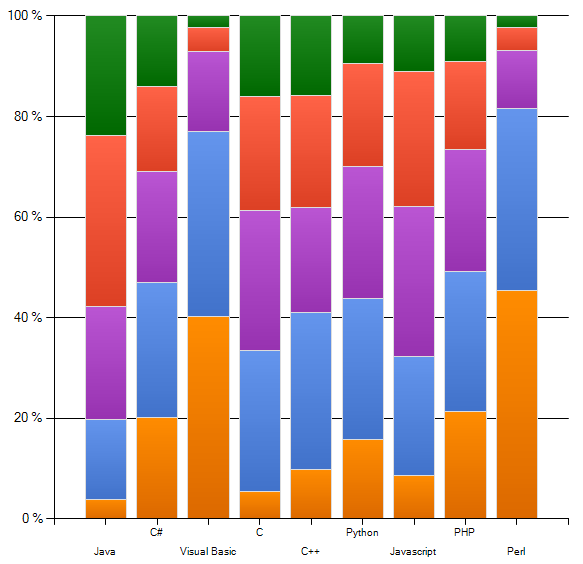
\includegraphics[width=3.5in,height=2in]{experience.png}
%%  \caption{Participant familiarity with various programming languages. Starting at bottom: None, Somewhat familiar, Familiar, Very Familiar, Expert.}
%%\end{figure}
%
%\subsection{Mockups}
%%\begin{figure*}
%%  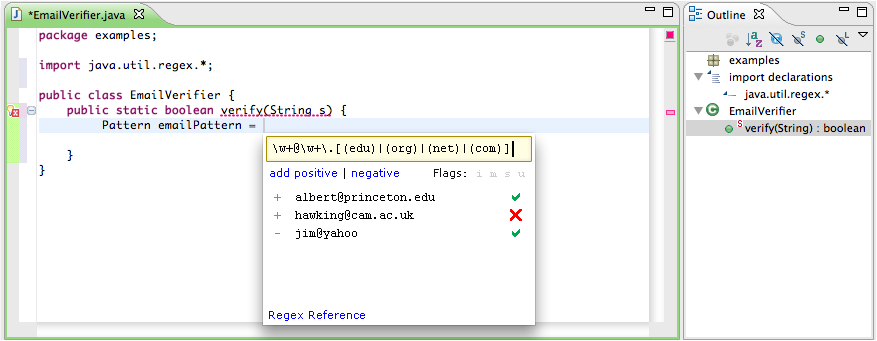
\includegraphics[scale=.6]{mockup-palette.png}
%%  \caption{The regular expression palette, shown in Eclipse.}
%%\end{figure*}
%Next, we presented participants with a series of mockup palettes corresponding to a Color class, a regular expression Pattern class (Figure 2) and a SQL query ResultSet class. In addition to a screenshot of the palette itself, participants were shown mockups demonstrating how a user would invoke the palette, and a mockup showing the code that would be inserted once a selection had been made. 
%
%Before presenting each palette mockup we gathered information about the user's familiarity with that topic and the strategies that they would likely use to instantiate that class. The Color class was presumed familiar to all participants. Figure 3 summarizes responses for the regular expression and SQL classes. The low number of participants unfamiliar with these topics again provides evidence that our participants were not generally novice developers.
%
%To determine the strategy typically used for instantiating the Color class, we asked the following question. The values in bold show the frequency of each response.
%
%\begin{quote}
%A user interface designer asks you to change the background color of a window to ``navy blue'' when the user presses a button. You have determined that you need to instantiate the 'Color' class to do so.
%\\\\
%Which of the following strategies would you use first to create an instance of the 'Color' class representing navy blue?\\
%
%\begin{enumerate}[(a)]
%\item I would use the IDE's content assist menu (see note below) to look for a predefined constant representing navy blue. (\textbf{58.4\%})
%\item I would look up the documentation of the Color class to see if there is a predefined constant representing navy blue. (\textbf{19.0\%})
%\item I would use an external tool (e.g. Photoshop or some other image editor) to determine the RGB values for navy blue. (\textbf{14.0\%})
%\item I would guess at the RGB values for navy blue, then check whether my guess was correct by executing the application. (\textbf{5.3\%})
%\item Other (please specify) (\textbf{3.3\%})\\
%\end{enumerate}
%\end{quote}
%
%Figure 4 summarizes the responses to a more general question asked about regular expressions and SQL queries.
%
%\begin{figure}
%\begin{tabular}{lccc}
% & \textbf{Regular Expressions} &  & \textbf{SQL}\\
% \hline
%Never used & 4.8\% &  & 0.0\%\\
%Use infrequently & 46.7\% &  & 37.4\%\\
%Use frequently & \textbf{48.4\%} &  & \textbf{62.6\%}\\
%\hline
%\end{tabular}
%\caption{Participant's experience with regular expressions and SQL.}
%\end{figure}
%
%\begin{figure}
%\begin{tabular}{lccc}
% & \textbf{Regular Expressions} &  & \textbf{SQL}\\
% \hline
%Separate test script & 29.7\% &  & 15.5\%\\
%Guess and check & 13.4\% &  & 16.0\%\\
%External tool & \textbf{38.5\%} &  & \textbf{58.9\%}\\
%Search for examples & 12.1\% & & 4.8\% \\
%Other & 6.2\% & & 4.8\% \\
%\hline
%\end{tabular}
%\caption{Typical strategies for regular expressions and SQL queries.}
%\end{figure}
%
%
%%For each of these classes,
%
%
%%\subsubsection{Color}
%%We began with a class representing colors. We asked participants to consider the following scenario:
%
%\begin{figure}
%\begin{tabular}{crccccc}\\\\
%\textsc{class}
%& 
%& \begin{rotate}{20}Nearly every time\end{rotate}
%& \begin{rotate}{20}Most of the time\end{rotate}
%& \begin{rotate}{20}Some of the time\end{rotate}
%& \begin{rotate}{20}Rarely\end{rotate}
%& \begin{turn}{20}Never\end{turn}\\
%\hline
%Color &\vline& 9.6\% & 22.1\% & \textbf{32.4\%} & 28.2\% & 7.7\%\\
%RegExp &\vline& \textbf{36.6\%} & 29.5\% & 21.8\% & 7.3\% & 4.8\%\\
%SQL & \vline &18.2\% & 19.3\% & \textbf{30.9\%} & 20.4\% & 11.4\%\\
%\hline
%\end{tabular}
%\caption{For each of the classes considered, participants were shown mockups of a code completion palette designed for instantiating that class, as well as the source code generated after parameters were entered. This table shows the distribution of responses to the question: ``Consider situations where you need to instantiate the [specified] class. What portion of the time, in these situations, do you think you would use this feature?''}
%\end{figure}
%%
%%\begin{figure}
%%  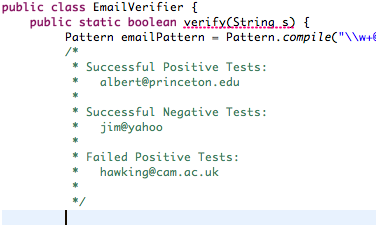
\includegraphics[scale=.6]{regex-insert.png}
%%  \caption{Test}
%%\end{figure}
%%
%%
%
%%Then we asked:
%%\begin{quote}
%%\textbf{Q2} Consider situations where you need to instantiate the 'Color' class. What portion of the time, in these situations, do you think you would use this feature?
%%\begin{enumerate}[(a)]
%%\item Nearly every time (\textbf{9.6\%})
%%\item Most of the time (\textbf{22.1\%})
%%\item Some of the time (\textbf{32.4\%})
%%\item Rarely (\textbf{28.2\%})
%%\item Never (\textbf{7.7\%})\\
%%\end{enumerate}
%%\end{quote}
%%
%
%After presenting each palette, we asked users to rate the usefulness of each palette. Responses are summarized in Figure 5. We then allowed participants to provide qualifications and open-ended feedback by asking the following question: ``If you would like to qualify or elaborate on your answer to the previous question you may do so below. You may also suggest improvements for this palette.'' This information is analyzed in the remainder of the paper.
%
%%\begin{quote}
%%\textbf{Q4} How would you describe your level of familiarity with (regular expressions, SQL)?\\
%%\\
%%\begin{enumerate}[(a)]
%%\item I do not know what [it is].	 (\textbf{0.7\%}, \textbf{0.0\%})
%%\item I know what regular expressions are but I have not used them in practice. (\textbf{4.4\%, 0.0\%})
%%\item I use regular expressions infrequently.	 (\textbf{46.0\%, 35.9\%})
%%\item I use regular expressions frequently. (\textbf{49.0\%, 64.1\%})
%%\end{enumerate}
%%\end{quote}
%
%
%
%%\begin{quote}
%%\textbf{Q5} Consider situations where you need to write a regular expression to extract information from a string or collection of strings. What strategy would you most likely use first?
%
%%\begin{enumerate}[(a)]
%%\item I would write a separate test script to help come up with an appropriate regular expression. (\textbf{29.7\%})
%%\item I would guess and check regular expressions by running my application. (\textbf{13.4\%})
%%\item I would launch an external application or web tool to help me test regular expressions interactively. (\textbf{38.5\%})
%%\item I would search the web for a sample regular expression suitable for my task. (\textbf{12.1\%})
%%\item Other (please specify) (\textbf{6.2\%})
%%\end{enumerate}
%%\end{quote}
%
%
%%\begin{quote}
%%\textbf{Q6} Consider situations where you need to create a regular expression. What portion of the time, in these situations, do you think you would use this feature?
%%\begin{enumerate}[(a)]
%%\item Nearly every time (\textbf{36.6\%})
%%\item Most of the time (\textbf{29.5\%})
%%\item Some of the time (\textbf{21.8\%})
%%\item Rarely (\textbf{7.3\%})
%%\item Never (\textbf{4.8\%})\\
%%\end{enumerate}
%%\end{quote}
%
%%\begin{quote}
%%\textbf{Q7} How would you describe your level of familiarity with SQL?
%
%%\begin{enumerate}[(a)]
%%\item I do not know what regular expressions are.	 (\textbf{0.0\%})
%%\item I know what SQL is I have not used it in practice. (\textbf{0.0\%})
%%\item I use SQL infrequently.	 (\textbf{35.9\%})
%%\item I use SQL frequently. (\textbf{64.1\%})\\
%%\end{enumerate}
%%\end{quote}
%
%%\begin{quote}
%%\textbf{Q8} Consider situations where you need to write a regular expression to extract information from a string or collection of strings. What strategy would you most likely use first?
%
%%\begin{enumerate}[(a)]
%%\item I would write a separate test script to help come up with an appropriate SQL query.	
% %(\textbf{15.5\%})
%%\item I would guess and check by running my application. (\textbf{16.0\%})
%%\item I would launch an external application or web tool to test my query against my database interactively.	(\textbf{58.9\%})
%%\item I would search the web for an example SQL query suitable for my task.	
% %(\textbf{4.8\%})
%%\item Other (please specify) (\textbf{4.8\%})
%%\end{enumerate}
%%\end{quote}
%
%%Showed the SQL palette and asked:
%
%%\begin{quote}
%%\textbf{Q9} Consider situations where you need to create a SQL query. How often, in these situations, do you think you would use this feature?
%%\end{quote}
%
%\section{Design Implications}
%%\begin{figure}[b]
%%  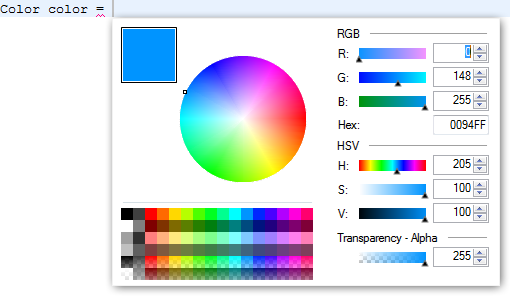
\includegraphics[scale=.5]{color-palette.png}
%%  \caption{test}
%%\end{figure}
%
%We next analyzed the open-ended responses to extract some design principles and constraints. We got 193 responses for the color palette, 129 for the regular expression palette, and 142 for the SQL palette. Also, we got total 119 suggestions about what other types of classes could benefit from similar types of palettes. The design can be divided into two main categories: system design constraints, and general palette design considerations. System design constraints are the criteria that should be taken into account in the design of the overall system architecture, and the general palette design considerations are about how to make more usable palettes.
%
%\subsection{System Design Constraints}
%
%\subsubsection{Handling Separation of Concerns}
%
%Professional developers were very wary of including constant data into the source code directly. Many responses expressed general sentiment or specific preference for project-wide color theme or external resource file. Also, many people stated that these tools might not be useful since they usually read an external resource file, or sometimes they explicitly suggested to add capability to handle the external resource files directly from the palette.
%
%Examples of feedbacks in this category include:
%
%\begin{itemize}
%	\item The use of magic numbers in the source code is a bad design (54)
%	\item Color picking is the `designer's job' (33)
%	\item Would only use to define named constants (17)
%	\item Would rather use color scheme / theme (3)
%	\item Would use Object-Relational Mapping (ORM) / Language INtegrated Query (LINQ) instead of raw SQL query string (27 of 142)
%	\item These palettes might be useful for prototyping, but not for real production (14)
%	\item Instead of including the test cases into comments, they should be stored as unit tests (35 of 143)
%\end{itemize}
%
%Interestingly, most people seemed to consider regular expressions as part of the program logic. There were few people who complained about including the regular expression pattern string in the source code.
% 
%\subsubsection{Reversibility}
%
%19 participants expressed that it should be able to bring the palettes back when they want to modify the parameters after they used the palettes.
% 
%\subsubsection{Palette Settings and State}
%
%Many participants wanted to be able to configure the palettes or have the palettes maintain state even after the palettes are hidden. The followings are the comments that are related to this category.
%
%\begin{itemize}
%	\item Want recently used regular expressions, and control over the comments (12)
%	\item Persistent database connection information is needed / want to manage connection pools (9)
%	\item Want recent colors, capability of setting favorite colors (20)
%\end{itemize}
%
%\subsubsection{Interaction with Code Context}
%
%Some people wanted to interact with the code context. For example, 13 people expressed that it would be great if the SQL query palette was capable of dynamically creating SQL query string by combining multiple string variables, or by assigning variables for the parameters.
%
%\subsubsection{Performance}
%
%Developers were concerned about the performance of these palettes. Some of the participants said that they would use these palettes only if it does not slow down the IDE. Also, this was the most popular comment on the reddit thread.
%
%\subsubsection{IDE Independence}
%
%Several participants expressed a desire for IDE or even language independence for these palettes.
%
%%\subsubsection{Composing palette logic}
%
%\subsection{General Palette Design Considerations}
%\subsubsection{Simplicity vs. Capability}
%
%Even though the participants were shown the same mockup screenshots, their reactions were split. Our color palette was considered too complex by many participants (26), and many others (26) would be satisfied with seeing colors next to a list of color names. The regular expressoin palette and SQL palette were considered too simple (12, and 15 participants respectively). They wanted syntax highlighting, match highlighting, and browsing capability of SQL databases.
%
%\subsubsection{Keyboard Navigability}
%
%12 of the participants expressed strong antipathy toward the mouse. This was mostly directed at the color palette.
%
%\subsubsection{Complexity}
%
%%\subsubsection{Side Effects}
%
%\section{Suggestions from the Participants}
%We classified the suggestions into several categories. The number in the parentheses indicate the number of participants who suggested the classes which fall into the category.
%
%\subsection{Alternative/Tricky/Literal Syntax (16)}
%These are the classes of which syntax is tricky, or complex. Even for a basic string class, people wanted to input multiline string or unicode string in more convenient way with automatic escaping.
%
%\begin{itemize}
%	\item Example classes
%	
%	\begin{itemize}
%		\item String
%		\item Collections (e.g., dictionary)
%		\item Vector, Matrix
%		\item Embedded languages
%		\item URLs, Paths
%	\end{itemize}
%	
%	\item Expected features
%	
%	\begin{itemize}
%		\item Proper escaping
%		\item Syntax highlighting
%		\item Auto-completion
%	\end{itemize}
%\end{itemize}
%
%\subsection{Unclear Parameter Implications (11)}
%The classes in this category has some parameters in it, and it is not easy to predict the results of the parameter modifications. Instead of running the whole application to see the result, the palette can serve as a preview panel so that the developers may check the results directly. Also, the palette can be a control panel which facilitates modifying the parameters.
%\begin{itemize}
%	\item Example classes
%	
%	\begin{itemize}
%		\item Audio tweaks (modifying pitch, volume, etc.)
%		\item 3D transformation matrices
%		\item number / string / date formatting
%		\item message box / input box (e.g., \texttt{JOptionPane})
%	\end{itemize}
%\end{itemize}
%
%\subsection{Query Languages (17)}
%Similar to the unclear parameter implications category, the developers wanted to check if the query string is correct or not by checking the results directly on the palette.
%
%\begin{itemize}
%	\item Example classes
%	
%	\begin{itemize}
%		\item Regular expression
%		\item SQL query
%		\item XPath / XQuery
%	\end{itemize}
%\end{itemize}
%
%\subsection{Graphical Elements (27)}
%The other popular category was graphical elements. We've already shown the color example, and the participants suggested many other graphical properties such as font, brush, shape and others. Also, people wanted to check or directly manipulate the GUI frames and layouts.
%
%\begin{itemize}
%	\item Example classes
%	
%	\begin{itemize}
%		\item Color, Shape, Brush, Font, etc.
%		\item JFrame, Layouts, any swing components
%	\end{itemize}
%\end{itemize}
%
%\subsection{Complex Instantiation Procedures (5)}
%Some of the participants pointed out that these palettes might be useful to create an object which requires complex instantiation code. For example, in order to read a text file in Java, the developer might want to use \texttt{BufferedReader} class. The instantiation code might look as following:
%\begin{verbatim}
%BufferedReader reader = null;
%try {
%    reader = new BufferedReader(
%        new FileReader(filePath));
%} catch (IOException e) {
%    e.printStackTrace();
%}
%// use reader here
%reader.close();
%\end{verbatim}
%By using a palette to choose a file or choose a variable which contains the file path, the developers could easily instantiate these objects. In the same way, it can alleviate the factory pattern usability problem. As long as the developers remember which class to use, they will not need to remember how to instantiate that class.
%
%\begin{itemize}
%	\item Example classes
%	
%	\begin{itemize}
%		\item BufferedReader
%		\item Classes using factory patterns
%		\item Database connection string builder
%	\end{itemize}
%\end{itemize}
%
%\subsection{Describe by Example (2)}
%Sometimes, it is possible to describe an object by examples. For instance, if there is a class which represents a shortcut key combination, we can easily instantiate an object of that class by pressing the actual shortcut key on the interactive palette.
%
%\begin{itemize}
%	\item Example classes
%	
%	\begin{itemize}
%		\item Keyboard Keys
%		\item Regular expression
%	\end{itemize}
%\end{itemize}
%
%\subsection{Integrating with Documentation, Tutorial (7)}
%Some participants suggested integrating the documentation or the tutorials into the interactive palettes. If the developers are not familiar of the specific API class, the palette could tell them how to use it.
%
%%\begin{itemize}
%%\item 54 expressed a concern about encouraging inlining of constants, preferring external resource files. 17 stated that they would use this feature only to define constants. 33 stated that it should be the designer's job.
%%\item 11 expressed a concern about keyboard navigability
%%\item 27 expressed a concern about the complexity of the palette
%%\item 10 expressed an interest in a color picker. 7 wanted a multitabbed window with different options for picking colors.
%%\item 26 expressed a desire for color names, 10 of which wanted to ensure color constant names were used if available
%%\item 20 wanted persistent state (MRU, favorites)
%%\end{itemize}
%
%% An example of a floating figure using the graphicx package.
%% Note that \label must occur AFTER (or within) \caption.
%% For figures, \caption should occur after the \includegraphics.
%% Note that IEEEtran v1.7 and later has special internal code that
%% is designed to preserve the operation of \label within \caption
%% even when the captionsoff option is in effect. However, because
%% of issues like this, it may be the safest practice to put all your
%% \label just after \caption rather than within \caption{}.
%%
%% Reminder: the "draftcls" or "draftclsnofoot", not "draft", class
%% option should be used if it is desired that the figures are to be
%% displayed while in draft mode.
%%
%%\begin{figure}[!t]
%%\centering
%%\includegraphics[width=2.5in]{myfigure}
%% where an .eps filename suffix will be assumed under latex, 
%% and a .pdf suffix will be assumed for pdflatex; or what has been declared
%% via \DeclareGraphicsExtensions.
%%\caption{Simulation Results}
%%\label{fig_sim}
%%\end{figure}
%
%% Note that IEEE typically puts floats only at the top, even when this
%% results in a large percentage of a column being occupied by floats.
%
%
%% An example of a double column floating figure using two subfigures.
%% (The subfig.sty package must be loaded for this to work.)
%% The subfigure \label commands are set within each subfloat command, the
%% \label for the overall figure must come after \caption.
%% \hfil must be used as a separator to get equal spacing.
%% The subfigure.sty package works much the same way, except \subfigure is
%% used instead of \subfloat.
%%
%%\begin{figure*}[!t]
%%\centerline{\subfloat[Case I]\includegraphics[width=2.5in]{subfigcase1}%
%%\label{fig_first_case}}
%%\hfil
%%\subfloat[Case II]{\includegraphics[width=2.5in]{subfigcase2}%
%%\label{fig_second_case}}}
%%\caption{Simulation results}
%%\label{fig_sim}
%%\end{figure*}
%%
%% Note that often IEEE papers with subfigures do not employ subfigure
%% captions (using the optional argument to \subfloat), but instead will
%% reference/describe all of them (a), (b), etc., within the main caption.
%
%
%% An example of a floating table. Note that, for IEEE style tables, the 
%% \caption command should come BEFORE the table. Table text will default to
%% \footnotesize as IEEE normally uses this smaller font for tables.
%% The \label must come after \caption as always.
%%
%%\begin{table}[!t]
%%% increase table row spacing, adjust to taste
%%\renewcommand{\arraystretch}{1.3}
%% if using array.sty, it might be a good idea to tweak the value of
%% \extrarowheight as needed to properly center the text within the cells
%%\caption{An Example of a Table}
%%\label{table_example}
%%\centering
%%% Some packages, such as MDW tools, offer better commands for making tables
%%% than the plain LaTeX2e tabular which is used here.
%%\begin{tabular}{|c||c|}
%%\hline
%%One & Two\\
%%\hline
%%Three & Four\\
%%\hline
%%\end{tabular}
%%\end{table}
%
%
%% Note that IEEE does not put floats in the very first column - or typically
%% anywhere on the first page for that matter. Also, in-text middle ("here")
%% positioning is not used. Most IEEE journals/conferences use top floats
%% exclusively. Note that, LaTeX2e, unlike IEEE journals/conferences, places
%% footnotes above bottom floats. This can be corrected via the \fnbelowfloat
%% command of the stfloats package.
%
%
%
%\section{Conclusion}
%Overall, professional developers appear willing to use these for a number of use cases. However, the usability criteria described above impose stiff requirements on the architecture. Of particular concern, we found that the developers preferred help with program logic, but not the constant data. This indicates that another area of application may be in specialized editors for resource files.
%
%
\section{System Design and Implementation}
After completing the survey, we built an active code completion system named Graphite, an acronym for {\bf Gra}phical {\bf P}alettes to {\bf H}elp {\bf I}nstantiate {\bf T}ypes in the {\bf E}ditor. 
We chose to build the system as an extension to Eclipse for Java because this combination was the most widely-used  amongst participants in our survey. In the subsections below, we describe how several novel design decisions made it possible to satisfy design criteria from Section III and enabled several use cases described in Section IV. The end result is a simple system that allows an API's developers, as well as external developers, to build rich HTML5-based palettes that can be associated with both in-built and user-defined classes directly. Developers using an API can discover and invoke these palettes through the standard code completion menu.

\subsection{HTML5-Based Palettes}
Palette developers build palettes using HTML5 technologies (HTML, CSS and JavaScript). We made this decision for several reasons. 
Eclipse is written in Java and uses the SWT and JFace graphical user interface toolkits, but these are not widely used outside of the Eclipse ecosystem. JavaScript was among the most well-known languages in our study, just behind Java, C and C++, and is highly flexible. A number of useful libraries are available (e.g. jQuery \cite{jQuery}.) 

As noted in Section IV-H, a number of participants in our field study indicated that they hoped that our tool would be available for other IDEs and other programming languages. All major windowing toolkits feature a web browser control, so HTML5-based palettes can easily be loaded by different editor environments without developer intervention.

Deploying palettes using standard URLs is also simpler than attempting to integrate them directly into Java libraries and packages. It also eases the process of incremental and rapid development, as all major browsers now feature sophisticated debuggers and run-time inspection facilities. 

\subsection{Palette API}
Palettes communicate with the host IDE using a simple Javascript API. To access this API, the palette must include a small script named \verb|graphite.js| into their page. The default implementation of this script provides an implementation of the API methods for testing in a standard web browser. When loaded into an editor, the editor plug-in replaces these methods with specialized implementations. The API consists of the following methods, accessed through a global object named \verb|graphite|:
\begin{itemize}
	\item \verb|insert(str)|: Inserts the specified string at the cursor and closes the palette. The indentation is automatically inserted after any newlines in this string.
	
	\item \verb|cancel()|: Closes the palette without inserting code. Note that the ESC key cancels by default, and palettes are modal so clicking outside a palette will not cancel.
	
	\item \verb|getSelectedText()|: Returns the text that is currently selected in the editor, or an empty string if no text has been selected. This method is used to implement reinvocation -- users simply select previously generated code and invoke the palette as described in Section I. The palette is responsible for parsing the selected text to extract relevant parameters.
	
	\item \verb|getIDE()|, \verb|getLanguage()|: Return a string that specifies the IDE and language that is being used, ``Eclipse'' and ``Java'' in our implementation.
\end{itemize}

By limiting the complexity of this API, we reasoned that developers would be able to create specialized palettes more easily. A simple hello world palette is only two lines of code, for example. An additional benefit is that the developers of other editing environments should also be able to create plug-ins that support Graphite palettes with minimal effort.

\subsection{Palette Discovery}
\begin{figure*}\begin{center}
\vspace{2mm}
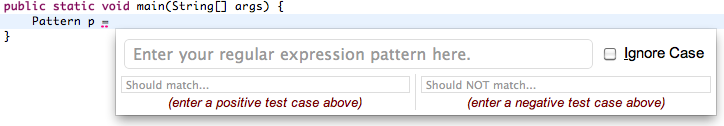
\includegraphics[scale=.6]{regex.png}\end{center}
\caption{The regular expression palette developed using Graphite and used by subjects in the treatment group of the user study described in Sec. VI.}
\end{figure*}

Graphite currently provides two methods for associating a palette with a particular class so that the editor plug-in can include it in the code completion menu when relevant.

\subsubsection{Annotation-based}
For user-defined classes that the palette developer has the authority to modify, the \texttt{@GraphitePalette} annotation associates a palette with the class. The annotation must specify the URL of the palette, and can contain some other optional information (e.g. the description that is shown in the code completion menu). This  allows API providers to provide palettes that are specialized to their libraries and distribute them directly alongside their code. The benefit of this approach is that users of the API are not required to discover that an external tool exists and explicitly install it into their IDE.

\subsubsection{Explicit}
In cases where a palette developer cannot modify a class directly (such as palettes for classes in the Java standard library), end-users can explicitly associate a palette with the fully qualified name of a class via a preference pane in the Eclipse IDE.

\subsection{Design Trade-Offs}
The design that we have described is light-weight, highly flexible and does not significantly impact IDE responsiveness. It also lays foundations for IDE and language portability. However, this design also leads to trade-offs:

\begin{itemize}
\item Because palettes are implemented in Javascript, any differences between the semantics of Java and Javascript can be problematic. For example, color names are slightly different between Java and Javascript, as are the regular expression engines. Although a Java applet could be used in cases where these differences are critical, this is still more difficult than it would be if the palettes were implemented in the same language.
\item The palette user interface must stay within its bounding box -- user interface elements like pop-up menus (unless they are provided by the browser itself) are thus more difficult to implement and may require additional API support in the future.
\item Several use cases could benefit from greater access to the surrounding code, or even the surrounding project. Implementing this modularly is particularly difficult, and the Eclipse API does not easily allow for  serialization of the sum of its contextual knowledge for consumption by a palette.
\item Because the reinvocation mechanism relies on parsing the selected code, the burden is high for both palette developers (although Javascript libraries for parsing Java code are available) and palette users. A better solution would be one where palette-related metadata is stored directly with the generated code. This could be partially addressed by the use of special comments to delimit sections of generated code and store palette metadata, but a more elegant solution would require a  change in how Java source code is represented.
\end{itemize}

%\section{Future work}
%
%\subsection{Graphite plug-in for different IDEs}
%As all the palettes are independent to Eclipse, We speculate that implementing Graphite plug-in for other IDEs will not be too difficult. Implementing a web-based aiding tool and sharing that tool among different IDEs with minimal effort will be a good idea.
%
%\subsection{Improving the Graphite API for Javascript}
%The current version of Graphite API for Javascript is not powerful enough. For example, the palettes cannot add comments before current line, nor can it delete or replace code fragment which was not highlighted by the user. By providing more effective and powerful API, the palette writers can write the palettes more quickly and make more useful palettes.
%
%\subsection{More palette examples}
%Due to the limited time, we could only provide two example palettes so far. More palette examples for various types might inspire the library providers and palette writers to design better palettes.
%
%\subsection{Keyword invocation model / online palette repository}
%Although Keyword invocation has many expected benefits, it is currently not supported. This model will make Graphite language-independent, and improve discoverability of the palettes by allowing users to search the palette with keywords. Palette search will work better if a shared online palette repository is built and maintained.
%
%


% An example of a floating figure using the graphicx package.
% Note that \label must occur AFTER (or within) \caption.
% For figures, \caption should occur after the \includegraphics.
% Note that IEEEtran v1.7 and later has special internal code that
% is designed to preserve the operation of \label within \caption
% even when the captionsoff option is in effect. However, because
% of issues like this, it may be the safest practice to put all your
% \label just after \caption rather than within \caption{}.
%
% Reminder: the "draftcls" or "draftclsnofoot", not "draft", class
% option should be used if it is desired that the figures are to be
% displayed while in draft mode.
%
%\begin{figure}[!t]
%\centering
%\includegraphics[width=2.5in]{myfigure}
% where an .eps filename suffix will be assumed under latex, 
% and a .pdf suffix will be assumed for pdflatex; or what has been declared
% via \DeclareGraphicsExtensions.
%\caption{Simulation Results}
%\label{fig_sim}
%\end{figure}

% Note that IEEE typically puts floats only at the top, even when this
% results in a large percentage of a column being occupied by floats.


% An example of a double column floating figure using two subfigures.
% (The subfig.sty package must be loaded for this to work.)
% The subfigure \label commands are set within each subfloat command, the
% \label for the overall figure must come after \caption.
% \hfil must be used as a separator to get equal spacing.
% The subfigure.sty package works much the same way, except \subfigure is
% used instead of \subfloat.
%
%\begin{figure*}[!t]
%\centerline{\subfloat[Case I]\includegraphics[width=2.5in]{subfigcase1}%
%\label{fig_first_case}}
%\hfil
%\subfloat[Case II]{\includegraphics[width=2.5in]{subfigcase2}%
%\label{fig_second_case}}}
%\caption{Simulation results}
%\label{fig_sim}
%\end{figure*}
%
% Note that often IEEE papers with subfigures do not employ subfigure
% captions (using the optional argument to \subfloat), but instead will
% reference/describe all of them (a), (b), etc., within the main caption.


% An example of a floating table. Note that, for IEEE style tables, the 
% \caption command should come BEFORE the table. Table text will default to
% \footnotesize as IEEE normally uses this smaller font for tables.
% The \label must come after \caption as always.
%
%\begin{table}[!t]
%% increase table row spacing, adjust to taste
%\renewcommand{\arraystretch}{1.3}
% if using array.sty, it might be a good idea to tweak the value of
% \extrarowheight as needed to properly center the text within the cells
%\caption{An Example of a Table}
%\label{table_example}
%\centering
%% Some packages, such as MDW tools, offer better commands for making tables
%% than the plain LaTeX2e tabular which is used here.
%\begin{tabular}{|c||c|}
%\hline
%One & Two\\
%\hline
%Three & Four\\
%\hline
%\end{tabular}
%\end{table}


% Note that IEEE does not put floats in the very first column - or typically
% anywhere on the first page for that matter. Also, in-text middle ("here")
% positioning is not used. Most IEEE journals/conferences use top floats
% exclusively. Note that, LaTeX2e, unlike IEEE journals/conferences, places
% footnotes above bottom floats. This can be corrected via the \fnbelowfloat
% command of the stfloats package.

\subsection{Palettes}
We implemented two palettes using the jQuery library for basic functionality \cite{jQuery}, which we used in the pilot study described below.

\subsubsection{Color Selection}
The color selection palette we ultimately developed was significantly simpler than the one shown in the preliminary survey, due to user comments. It allows users to enter any valid CSS color string, satisfying the requirements for keyboard navigability. The entered color is syntax checked and a preview is shown. Standard Java colors are also available as swatches that can be selected by the mouse if desired. Reinvocation support is provided. This palette took about 500 lines of code and markup, not including the jQuery library. Much of this was needed to translate arbitrary CSS color strings into RGB values, rather than for user interface logic.

\subsubsection{Regular Expressions}
Writing correct regular expression patterns is difficult. The regular expression palette, associated with the \verb|Pattern| class in the Java standard library, allows users to enter and test regular expression patterns interactively before inserting them into their code.  The focal point of this palette is the pattern input area. As the user enters a pattern into this input area, syntax errors are indicated with a red background; the background remains white when the pattern is valid.

In addition to the pattern, a regular expression consists of flags that can change its matching behavior in various ways. Our palette allows users to toggle the case-sensitivity flag of the regular expression using a small checkbox labeled \verb|Ignore Case|, placed next to the input area. A keyboard shortcut is also available, indicated using the underlined letter (Ctrl+I). 

To allow users to test the behavior of the regular expression that they have entered, two columns are available below the expression input area. The left column contains an input area labeled ``Should match...'' and the right column contains an input area labeled ``Should NOT match...''. Users use these to enter lists of test  strings into each column. The background colors behind these strings change to indicate whether the regular expression that has been entered matches or does not match that string. Green indicates that the pattern  {\it matched} the string and red indicates that it does {\it not} match, regardless of the column that the test is in (this scheme was chosen based on feedback from an initial pilot of this palette, the results of which are not included below.) A key describing this color scheme is displayed after the first test has been entered (not shown above, see video).

Users can navigate the palette using the keyboard using standard \verb|Tab| cycling behavior. The label in each text area remains visible until some input has been entered, rather than disappearing immediately on focus. When a user is satisfied with the regular expression that they have entered, she can press the \verb|Enter| key to insert the appropriate Java source code. Because Java requires that the regular expression pattern be placed inside a string literal, additional escape sequences are needed in front of backslashes. This can be tedious and error-prone if done manually. The palette automatically inserts these escape sequences. In addition to the source code itself, the tests are retained in a comment beginning on the next line. If the user wishes to modify the regular expression or change the test set, she can highlight the code that was inserted and then invoke the palette once again. The palette parses the selected text to extract the regular expression and tests.

This palette required about 700 lines of code and markup.

\section{Pilot Study}

We conducted a small controlled pilot study to evaluate the usefulness and usability of the Graphite system for a specific development task -- writing regular expressions -- and found significant benefits for the treatment group.

\subsection{Study Methods}
\subsubsection{Between-Subjects Design}
We used a between-subjects design by randomly assigning the participants to either the control group or the treatment group. In the control group, subjects were not shown or able to use any palettes. In the treatment group, subjects were shown the simple color palette shown in Figure 1, and allowed to discover and use the regular expression palette shown in Figure 5 if they wished. No specific training on the use of this palette was provided, to simulate realistic usage scenarios.

We chose a \textit{between-subjects design} because a within-subjects design would have required us to produce pairs of tasks with equal difficulties. This turned out to be very challenging. Second, we could not easily ignore a learning effect during the experiment if we had used a within-subjects design. We observed that this effect was quite strong, as most subjects had not used regular expressions recently.

\subsubsection{Training}
Only the participants in the treatment group were shown how to invoke Graphite palettes in the context of an  Eclipse code editor with a palette for the Color class. We chose to demonstrate the tool using a color palette instead of the regular expression palette itself because we wanted to simulate the condition where a user had discovered the palette naturally. The demonstration of the Color palette was brief, taking about two minutes.
We then described the nature of the task to the subject and allowed them to begin, giving them 45 minutes to complete all tasks, in any order.

\subsubsection{Tasks}

There were a total of 9 tasks to be completed in 45 minutes. The first 6 tasks involved writing regular expressions to validate various data formats (e.g. temperatures), and the remaining 3 tasks involved writing regular expressions to retrieve data from a document. The participants were allowed to move back and forth while doing the experiment, and they were allowed to use any external resources, including the internet, local console, and so forth (we did not observe any usage of programs other than the web browser, however). The only restriction we placed on their activity was that they were NOT allowed to directly search for the answer to a task online. We omit descriptions of each individual question due to space limitations.

\subsection{Participants}

We recruited 7 PhD students from CMU. The subjects were randomly assigned into two groups: 4 subjects were assigned to the control group, and the other 3 subjects to the treatment group. There were six male participants and one female participant. Participants were compensated in the amount of 15 dollars for their participation.

All subjects had prior experience with both Java and regular expressions, assessed using a preliminary survey similar to the one described in Section II.  Of note, the subjects in this study were slightly less skilled with Java and regular expressions than in the previous survey. This is consistent with the responses of the PhD students who participated in the online survey, who were also slightly less experienced on average. The only other significant difference in responses was that the PhD students were slightly less likely to prefer the use of external tools. The difference in the case of regular expressions was 13\%.

\subsection{Hypotheses}
In designing the regular expression palette, we had hypothesized that users would experience difficulties with two particular aspects of the Java Pattern API: that it used a factory pattern for instantiation, as opposed to the standard instantiation construct \cite{ellis_factory_2007}, and that it required special care with escape sequences -- escape sequences in the pattern must themselves be escaped, because the regular expression is written as a Java string literal. We observed difficulties with both of these issues in the control group, but not in the treatment group. The treatment group also completed more tasks than the control group on average (7 vs. 6.) The behaviors observed in these groups are described below.

\subsection{Preliminary Reading}
All subjects were somewhat rusty on the details of the Java Pattern API. After reading the prompt for the first task, all subjects began by searching for and reviewing documentation related to regular expressions. In all but one of these cases, the subject looked at the API documentation for the Java Pattern class during this initial review. The remaining subject, a member of the control group, referred to quick reference documentation provided by an external tool. In all cases, the documentation was left accessible in a browser window throughout the study, often displayed simultaneously alongside the coding window due to the large screen available for the study.

%
%\begin{itemize}
%	\item Data format validation tasks (total 6 tasks)
%	
%	\begin{enumerate}
%		\item US phone numbers
%		
%		For simplicity, it was assumed that any digit can be used in any place in the phone number, even though there is a notion of valid range for the area code.
%		
%		\item Times
%		
%		Hours and minutes only.
%		
%		\item Temperatures
%		
%		Only Fahrenheit and Celcius were used, and subjects were instructed to assume the degree symbol had not been used.
%		
%		\item Dates
%		
%		We did not place any restrictions on the format for dates. This task is quite difficult to solve generally. There are many valid formats for expressing dates, and the valid range of the day part depends on the specific year and month. Many participants were stuck on this task and chose to skip it and came back later.
%		
%		\item IPv4 addresses
%		
%		\item URLs starting with \texttt{http://} or \texttt{https://}
%		
%	\end{enumerate}
%	
%	\item Data searching tasks (total 3 tasks)
%	
%	\begin{enumerate}
%	\setcounter{enumi}{6}
%		\item Finding a fields declaration (member variable) in a Java class
%		
%		It was assumed that all the field declarations start with one of the access modifier keywords: \verb|public|, \verb|protected|, or \verb|private|.
%		
%		\item Finding a string literal in a Java file
%		
%		\item Finding an \texttt{img} tag in an HTML file
%		
%	\end{enumerate}
%	
%\end{itemize}
%
%\subsubsection{Task Structure}


%\begin{figure}[h]%
%\includegraphics[width=\columnwidth]{Task1.png}%
%\caption{The initial content of \texttt{Task1.java} file}%
%\label{task1}%
%\end{figure}


\subsection{Control Group}
In our previous online survey, we had found that no single strategy for writing regular expressions dominated the others.  We observed each of the common strategies -- use of external tools, test scripts and guess-and-check.

One subject began by using an external tool called regexpal.com. After writing a full regular expression and attempting to test it using the tool, the subject became dissatisfied with it and switched to a different tool, regextester.com. This tool too appeared to be unsatisfactory, as all subsequent tasks were performed without the aid of external tools or tests.

The other subjects chose to write their regular expressions directly within Eclipse from the beginning. One of these subjects never compiled or checked the accuracy of the regular expressions beyond making sure Eclipse errors were addressed, while the other two attempted to write Java stubs within the test files to test the regular expression that they had written. They experienced considerable difficulty with this task, with one subject taking over 10 minutes to write the test code. The code could only check one example at a time and the subject used it to check a single positive example per task.

One of the four control subjects tried the \verb|new Pattern| construct. An Eclipse error alerted the subject to the problem shortly thereafter. After referring to an example in the inline API documentation for the class, the subject was able to correct this error. The remaining subjects all noticed this example beforehand, and were able to avoid this problem.

Three of the four control subjects experienced significant difficulties associated with escape sequences. One subject recognized the error fairly quickly after Eclipse complained that the escape sequences used in the pattern were invalid (they were, in fact, valid escape sequences for regular expression patterns, but not for string literals.) The subject continued to miss escape sequences occasionally throughout the remainder of the study, but was able to fix them quickly after Eclipse alerted the subject to the error. For the other two subjects, the problem was more severe. In both cases, they noticed the error that Eclipse gave, but thought it indicated a problem with their pattern itself. One subject thought that the uses of symbolic escape sequences like \verb|\(| were incorrect. He decided to replace these with ASCII escape sequences (\verb|\050|) after looking up an ASCII conversion table. This was an unnecessary and overly complex solution to the problem. The other subject thought that the problem was in his use of the whitespace escape sequence, \verb|\s|. Thus, he  spent several minutes looking up how to match whitespace correctly. In doing so, he found a description of the double-escape problem in Java and fixed the problem after that.
\subsection{Treatment Group}
One subject was already familiar with an external tool, regexpal.com (also used by a subject in the control group), and used it variously throughout the task. In most cases, the subject used the external tool's quick reference documentation while using our palette for authoring and testing. At other times, the subject used the external tool itself. The subject indicated that in some cases, he was not sure that our palette was free of bugs (when something unexpectedly matched or did not match. We did not observe any actual errors related to regex matching in our tool, however.), and also because the external tool provided syntax and substring highlighting, a useful feature for complex regular expressions. When done with the external tool, the subject pasted the pattern into our tool to generate the appropriate code. As such, the subject had no difficulties with escaping or factory pattern instantiation.

The other two subjects in the treatment group did not use any external tools. Both subjects decided not to use our palette for the first task (likely because they forgot that it was available, since they spent some time looking up API documentation after our initial demo with the color palette.) They both recognized the need for the factory pattern and also both had an initial error related to escaping that they were able to resolve before moving on. One of these subjects also began to write tests within a \verb|main| method.

Beginning with the second task, both subjects remembered that a palette may be available and were able to invoke it correctly. They all recognized that the primary input box was where the regular expression should be entered and that the two other input boxes were for positive and negative tests, respectively. Two of the subjects did not initially realize that multiple tests could be entered, and that entering even a single test required pressing the \verb|Enter| key. One subject never fully understood this, relating after the study that he thought that the palette would notify him when he was done if the example that he had entered was not matched by the pattern. The other subject was able to use the test case input boxes correctly after initial experimentation. This was perhaps due to the wording of the prompts under these entry boxes: ``enter \textbf{a} [positive \verb1|1 negative] test case above''. This problem was corrected in a version of the palette developed following this study.

Two of the subjects used the reinvocation feature of the palette, but neither highlighted the test cases, meaning that they had to enter new test cases every time they reinvoked the palette. This may have been due to the fact that our example with the Color palette involved only a single line of text (unlike the example in Figure 1). The third subject never used this feature.

Two of the subjects expressed confusion about the meaning of the green and red backgrounds on the test cases. Although we provided a key saying that green meant that ``pattern matches string'', the headings of the two columns: ``[should \verb1|1 should NOT] match:'', may have caused confusion. We had changed the meaning of these colors due to feedback from our initial presentation of the tool, so it is clear that regardless of the interpretation given, some subjects were confused.

Despite these difficulties, however, the basic functionality of the palette seemed to help all of the subjects. None struggled with issues related to escaping and instantiation, for example. Although the sample size is not large enough to make many quantitative judgements, it was observed that the treatment group completed more of the tasks than the test group on average (7 tasks for the treatment group vs. 6 for the control group). All of the subjects in the treatment group, as well as members of the control group who were shown the palette after the study, indicated that they felt that the palette was helpful, and several provided specific suggestions for improvements.


%\section{Future Work}
%
%\subsection{Palette Design Improvements}
%The observations above suggest several potential improvements for the regular expression palette. Some of the problems appeared to be due to the subject's lack of familiarity with the Graphite system. In particular, subjects did not highlight the full text needed to reinvoke the palette, likely due to the the limited training protocol. By showing only a single, simple example, the subjects were not able to generalize the reversibility mechanism to multiline completions. If the training period had included such an example, we suspect that this would not have been a problem. 
%
%In other cases, more explicit labels in the palette may have helped. The subjects began by entering only a single example because the label on the palette used the singular article, ``a''. We suspect that we could have avoided this problem if the label was more explicit: ``Create positive examples by entering them above and pressing ENTER''. Confusion over the meaning of the green and red backgrounds may also have been avoided by using a clearer label for the key, accompanied by a label explaining the meaning of each column more explicitly.
%
%In conjunction with these improvements, it would be useful to have an explicit ``Help'' button that allowed users to view documentation or a training video for the palette. On first invocation, it may also have been helpful to invoke this video automatically (though this would require tool support for associating data with the user.)
%
%Several subjects suggested new features for the regular expression palette, including syntax highlighting, substring highlighting and an explicit option to match the whole string, rather than any part of the string (a problem encountered by several subjects in both groups). They also suggested including inline quick reference documentation and regex snippets directly within the palette. Other people (not a part of the study) have suggested other features, including a tool for building regular expressions directly from examples, and a tool for generating examples automatically from regular expressions. Examples of such tools exist online.
%
%\subsection{Study Design Improvements}
%
%Some of the limitations in our study design, combined with the small size of our subject pool, made any sort of quantitative analysis difficult. In this section, we suggest some possible improvements.
%
%	\paragraph{Task Difficulty} Subjects were sometimes ``stumped'' by some of the more difficult tasks. It would perhaps be helpful to remove some of these excessively difficult tasks. For example, validating US phone numbers and dates turned out to be much more difficult than the others.
%	
%	\paragraph{Giving a time limit for each task} Because we only imposed a time limit for the whole experiment, it was difficult to compare performance on an individual task, in terms of time spent. However, imposing a per-task time limit may introduce concerns about the learning effect -- most subjects spent a significant amount of time looking up documentation in the early part of the study. One possibility may be to introduce dummy tasks at the beginning of the experiment.
%	
%	\paragraph{Using other types of Graphite palettes} This study does not evaluate the whole Graphite plug-in architecture, and many of the issues may have been due to the regular expression task and palette specifically. Designing a study to effectively evaluate the design as a whole would likely require building several more high-quality palettes.
%	
%	[Evaluating performance] It is difficult to measure accuracy of provided regular expressions due to their inherent complexity. We could not run an automated test suite on the subject responses because many subjects had syntax errors or other problems in their final submission that would have caused trivial failures. 	Poor-quality regular expressions written in a relatively short amount of time may also be hard to compare to high-quality regular expressions written in a longer amount of time. 
%		

\subsection{Threats to Validity}
In addition to the small sample size and the sampling bias discussed earlier, subjects in the treatment group may have been biased to use our features due to their novelty (although two subjects did not use the palette until their second task). We only tested a regular expression palette, so other types of palettes may not necessarily be as useful, and this palette had significant flaws that were corrected only after this study.

\section{Related Work}
In addition to the code completion work discussed in the introduction, some other research areas are related to active code completion. 
\subsection{Active Libraries}
We named this technique {\it active code completion} because of its relation to the general concept of {\it active libraries} \cite{activelibraries}. Active libraries are libraries that contain program logic that is invoked at either compile-time or, here, design-time. 

\subsection{Visual Languages}
Because active code completion involves graphical user interface elements but ultimately generates textual source code representations, it can be considered a hybrid approach that borrows interaction techniques from visual languages while remaining compatible with conventional programming languages. This hybrid approach may help address some of the usability challenges previously associated with visual languages (cf. \cite{doi:10.1080/1049482940040202}).

Editing environments like Barista \cite{Ko06} and the RBA editor \cite{RBA} also merge concepts from both text-based and structured editors by allowing for alternative code representations within a relatively conventional layout. Barista provides the opportunity for rich type-specific interfaces, but it is an IDE generation framework, so new extensions require recompilation. The RBA editor focuses on code readability rather than new modes of interaction, but new registrations can be added relatively easily. Both tools use a custom domain-specific language, which is likely to be unfamiliar to many users. 

In future work, we hope to explore an extensible, keyboard-driven, code-generation based approach that leverages structured code representations to eliminate the difficulties associated with reinvocation and maintaining palette state described in this paper.

\subsection{Specific IDE Features}
There exist some IDE features that have been specifically designed for certain types. For example, CodeRush \cite{CodeRush} and Resharper \cite{Resharper} have color dialogs that allow developers to launch a color picker directly from the code editor. IntelliJ IDEA has an inline regular expression palette, driven by its Intentions system, as well \cite{IntelliJRegexp}. However, these IDE specific features are hard-coded -- user-defined types cannot provide similar functionality. Recent versions of Visual Studio support user-defined palettes associated with specific fields, rather than classes, of user interface widgets \cite{VSWidgets}. These are shown only in the property pane when using the graphical window layout editor.

\section{Conclusion}
Motivated by evidence that integrating highly-specialized tools directly into a developer's workflow is useful, we have developed the concept of active code completion as a generalization of conventional code completion. We validated the usefulness by generating a number of use cases and developed general design constraints for such tools, as well as the underlying architecture, by conducting an extensive survey of professional developers. Based on these findings, we developed Graphite, an active code completion architecture that makes several novel design decisions that ease the development, deployment and discovery of user-defined palettes. We created palettes for color and regular expression classes and validated the latter palette's usefulness with a pilot study, providing evidence for the more general claim that integrating palettes into code completion is useful. We claim that active code completion systems like Graphite will considerably ease this process.

\section{Availability}
Graphite is free, open-source software available from the URL on the first page. We encourage readers to install it and tell us about any interesting palettes that they develop.

% conference papers do not normally have an appendix


% use section* for acknowledgement
\section*{Acknowledgment}
{We would like to thank the participants in our survey and pilot study, Jonathan Aldrich, the PLAID group, the students of 05-899D, anonymous reviewers and the UIUC Software Engineering Seminar group for valuable feedback. 
This material is based upon work supported by the National Science Foundation under Grant No. CCF-0811610. CO is supported by a DOE CSGF under Grant No. DE-FG02-97ER25308, and YY is supported by the Korea Foundation for Advanced Studies.}

% trigger a \newpage just before the given reference
% number - used to balance the columns on the last page
% adjust value as needed - may need to be readjusted if
% the document is modified later
%\IEEEtriggeratref{8}
% The "triggered" command can be changed if desired:
%\IEEEtriggercmd{\enlargethispage{-5in}}

% references section

% can use a bibliography generated by BibTeX as a .bbl file
% BibTeX documentation can be easily obtained at:
% http://www.ctan.org/tex-archive/biblio/bibtex/contrib/doc/
% The IEEEtran BibTeX style support page is at:
% http://www.michaelshell.org/tex/ieeetran/bibtex/
%\bibliographystyle{IEEEtran}
% argument is your BibTeX string definitions and bibliography database(s)
%\bibliography{IEEEabrv,../bib/paper}
%
% <OR> manually copy in the resultant .bbl file
% set second argument of \begin to the number of references
% (used to reserve space for the reference number labels box)
\bibliographystyle{IEEEtran}
%\bibliography{graphite-icse12}
\balance \bibliography{../research}



% that's all folks
\end{document}


